\documentclass[a4paper,11pt,titlepage]{article}
\usepackage[english]{babel}
\usepackage[utf8]{inputenc}
\usepackage[T1]{fontenc}
\usepackage[a4paper,top=1in,bottom=1in,left=1in,right=1in,marginparwidth=1.75cm]{geometry}
\usepackage{pgfplots}
\pgfplotsset{compat=1.18}
\usepackage{afterpage}
\usepackage{amsmath}
\usepackage{amsthm}
\usepackage{amssymb}
\usepackage{csquotes}
\usepackage{enumitem}
\usepackage{graphicx}
\usepackage{booktabs}
\usepackage{listings}
\lstset{
    frame = single, 
    framexleftmargin=15pt
}
\usepackage{caption}
\captionsetup[figure]{labelfont={bf},labelsep=quad}
\usepackage[ruled,vlined]{algorithm2e}
\makeatletter
\renewcommand{\SetKwInOut}[2]{%
  \sbox\algocf@inoutbox{\KwSty{#2}\algocf@typo:}%
  \expandafter\ifx\csname InOutSizeDefined\endcsname\relax% if first time used
    \newcommand\InOutSizeDefined{}\setlength{\inoutsize}{\wd\algocf@inoutbox}%
    \sbox\algocf@inoutbox{\parbox[t]{\inoutsize}{\KwSty{#2}\algocf@typo:\hfill}~}\setlength{\inoutindent}{\wd\algocf@inoutbox}%
  \else% else keep the larger dimension
    \ifdim\wd\algocf@inoutbox>\inoutsize%
    \setlength{\inoutsize}{\wd\algocf@inoutbox}%
    \sbox\algocf@inoutbox{\parbox[t]{\inoutsize}{\KwSty{#2}\algocf@typo:\hfill}~}\setlength{\inoutindent}{\wd\algocf@inoutbox}%
    \fi%
  \fi% the dimension of the box is now defined.
  \algocf@newcommand{#1}[1]{%
    \ifthenelse{\boolean{algocf@inoutnumbered}}{\relax}{\everypar={\relax}}%
%     {\let\\\algocf@newinout\hangindent=\wd\algocf@inoutbox\hangafter=1\parbox[t]{\inoutsize}{\KwSty{#2}\algocf@typo\hfill:}~##1\par}%
    {\let\\\algocf@newinout\hangindent=\inoutindent\hangafter=1\parbox[t]{\inoutsize}{\KwSty{#2}\algocf@typo:\hfill}~##1\par}%
    \algocf@linesnumbered% reset the numbering of the lines
  }}%
\makeatother
\usepackage{bm}
\usepackage[normalem]{ulem}
\setlength{\marginparwidth}{2cm}
\usepackage[colorinlistoftodos]{todonotes}
\usepackage[colorlinks=true, allcolors=blue]{hyperref}
\renewcommand*{\rmdefault}{bch}
\renewcommand*{\ttdefault}{lmtt}
\newcommand{\citationneeded}{\textcolor{red}{[citation-needed]}}
\DeclareMathOperator*{\argmin}{\arg\!\min}
\DeclareMathOperator*{\argmax}{\arg\!\max}
\setlength{\parskip}{0.5em}
\usepackage[numbers, comma, square, sort&compress]{natbib}
\bibliographystyle{abbrvunsrtnat.bst}
\theoremstyle{definition}
\newtheorem{definition}{Definition}[section]
\theoremstyle{plain}
\newtheorem{theorem}{Theorem}[section]
\newtheorem{corollary}{Corollary}[theorem]
\newtheorem{lemma}[theorem]{Lemma}
\theoremstyle{remark}
\newtheorem*{remark}{Remark}
\newcommand{\reporttitle}{Scientific Machine Learning:\\Neural Differential Equations}
\newcommand{\reportauthorA}{Jiaru (Eric) Li (CID: 02216531)}
\newcommand{\reportauthorB}{Xinyan Wang (CID: 02205857)}
\newcommand{\reportauthorC}{James Tay (CID: 02015786)}
\newcommand{\reportauthorD}{Jiankuan Liu (CID: 02215415)}
\newcommand{\reportauthorE}{Tianshi Liu (CID: 02218664)}
\newcommand{\supervisor}{Sheehan Olver}
\begin{document}
\begin{titlepage}
\newcommand{\HRule}{\rule{\linewidth}{0.5mm}}

\includegraphics[width=8cm]{figures/Imperial_logo.png}\\[1cm]
\center
\textsc{\LARGE Imperial College London}\\[0.5cm] 
\textsc{\Large Department of Mathematics}\\[1.5cm] 
\textsc{\Large Second-year Group Research Project}\\[0.5cm]
\makeatletter
\HRule \\[0.6cm]
{\huge \bfseries \reporttitle}\\[0.6cm]
\HRule \\[1.5cm]
\begin{minipage}{0.4\textwidth}
\begin{flushleft} \large
\emph{Author:}\\
\reportauthorA \\
\reportauthorB \\
\reportauthorC \\
\reportauthorD \\
\reportauthorE
\end{flushleft}
\end{minipage}
~
\begin{minipage}{0.4\textwidth}
\begin{flushright} \large
\emph{Supervisor(s):} \\
\supervisor
\end{flushright}
\end{minipage}\\[2cm]
\makeatother
\vfill
\makeatletter
{\large \today}\\[2cm]
\makeatother
\end{titlepage}

\begin{abstract}

\end{abstract}

\tableofcontents

\section{Introduction}

\section{Basic Neural Networks}

\subsection{History}

Before diving into neural ordinary and control differential equations, we shall first explore the field of \textit{neural network}. Generally speaking, a neural network is a group of units called \textit{neurons} connected by signals called \textit{synapses}.

In 1943, Warren McCulloch and Walter Pitts published a seminal paper \cite{McCulloch1943}, in which they proposed the first mathematical model of an \textit{artificial neural network}, inspired by biological neural networks in animal brains. This model was named the McCulloch–Pitts neuron, or \textit{perceptron}. In some sense, it could ‘learn’ from given data and make decisions or predictions based on some parameters. The process of optimising the choice of such parameters is called \textit{training} the neural network.

Later in 1958, Frank Rosenblatt described an implementation of perceptron in detail \cite{Rosenblatt1958}. The field of neural network expanded quickly, and nowadays, it is extensively used in various fields such as machine learning and artificial intelligence. We shall explore some simple applications later.

\subsection{Concepts}

\subsubsection{Structure}

A neural network (abbreviated NN) consists of interconnected neurons, each of which can be thought of as a mathematical function. They are typically organised into \textit{layers} consisting of

\begin{itemize}
    \item an \textit{input layer} that receives the data,
    \item multiple \textit{hidden layers} that processes the data, and
    \item an \textit{output layer} that produces the result.
\end{itemize}

The input and output data are usually given as real numbers. Therefore, the whole neural network can be thought of as a function $f:\mathbb{R}^m\rightarrow\mathbb{R}^n$ that takes an input vector $\mathbf{x}$ of dimension $m$ and an output vector $\mathbf{y}$ of dimension $n$.

The ultimate purpose of training a neural network is to minimise the error between the predicted output $\mathbf{y}$ and the target output $\mathbf{\hat{y}}$, usually given as a \textit{loss function} $L(\mathbf{y}, \mathbf{\hat{y}})$. Each connection between neurons has a \textit{weight}, and possibly a \textit{bias}, which are adjusted in the process of training, allowing the model to generalise to unseen data. They are usually given altogether as a \textit{weight matrix} $\mathbf{W}$ and a \textit{bias vector} $\mathbf{b}$.

\subsubsection{Activation Function}

For neural networks with multiple layers, an \textit{activation function} $\sigma$ is usually used. This is because it helps to decide whether a neuron should be ‘activated’ and introduces non-linearity into the model. The output of each neuron in a layer is therefore calculated as $\mathbf{z}^l=\sigma\left(\mathbf{W}^l\mathbf{z}^{l-1}+\mathbf{b}^l\right)$, where $\sigma$ acts element-wise, $\mathbf{z}^l$ is the output vector for layer $l$, $\mathbf{W}^l$ is the weight matrix connecting layer $l-1$ to layer $l$, and $\mathbf{b}^l$ is the bias vector for layer $l$. 

As for the choice of the activation function, the S-shaped \textit{sigmoid function} has some nice properties: it is bounded, differentiable with a non-negative derivative, and has exactly one point of inflection. Two familiar examples of sigmoid functions are the \textit{logistic function} $\sigma(x)=1/\left(1+e^{-x}\right)$ and the hyperbolic tangent function $\sigma(x)=\tanh x$. Another commonly used activation function is the \textit{rectifier}, or \textit{rectified linear unit} (ReLU), defined as $\sigma(x)=\max(0, x)$.

\begin{figure}[htbp]
    \centering
    \begin{minipage}{0.32\textwidth}
        \centering
        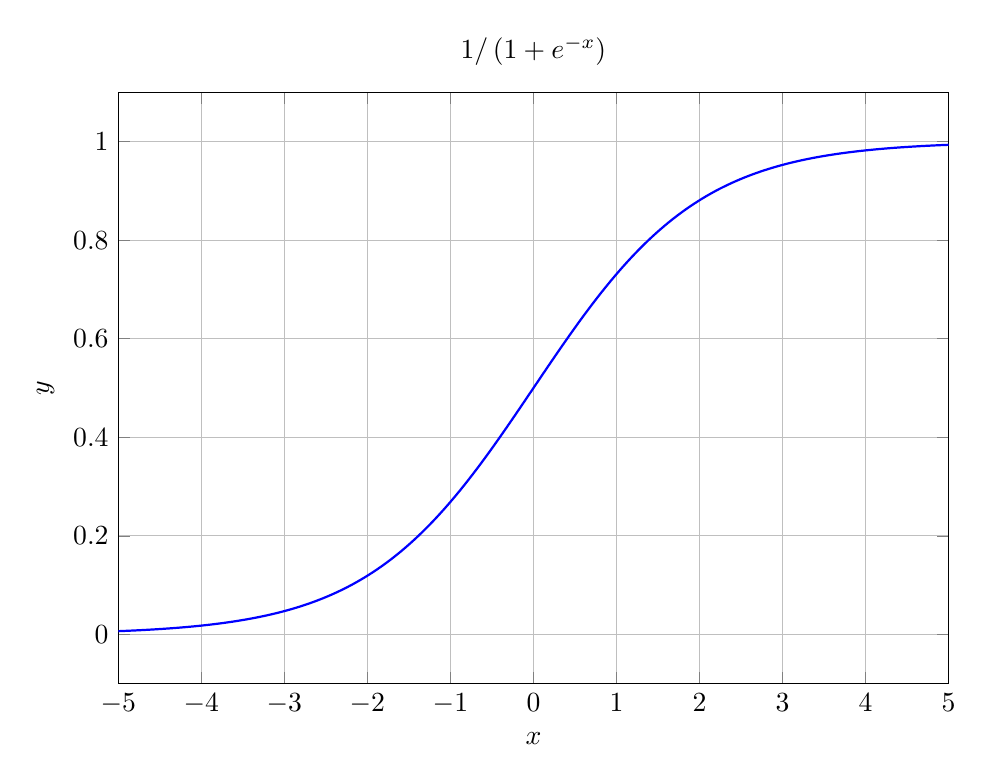
\begin{tikzpicture}
            \begin{axis}[
                title={$1/\left(1+e^{-x}\right)$},
                xlabel={$x$},
                ylabel={$y$},
                grid=major,
                width=\textwidth,
                height=0.75\textwidth,
                xmin=-5, xmax=5,
                ymin=-0.1, ymax=1.1,
            ]
                \addplot[blue, thick, samples=200] {1 / (1 + exp(-x))};
            \end{axis}
        \end{tikzpicture}
    \end{minipage}%
    \hfill
    \begin{minipage}{0.32\textwidth}
        \centering
        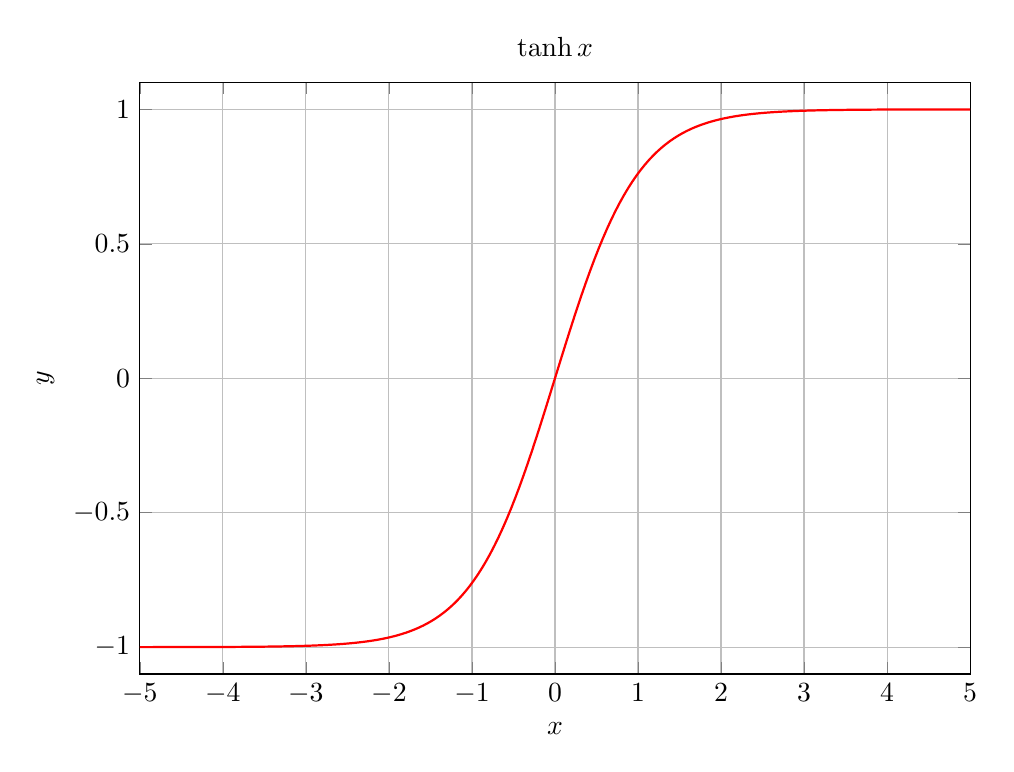
\begin{tikzpicture}
            \begin{axis}[
                title={$\tanh x$},
                xlabel={$x$},
                ylabel={$y$},
                grid=major,
                width=\textwidth,
                height=0.75\textwidth,
                xmin=-5, xmax=5,
                ymin=-1.1, ymax=1.1,
            ]
                \addplot[red, thick, samples=200] {tanh(x)};
            \end{axis}
        \end{tikzpicture}
    \end{minipage}%
    \hfill
    \begin{minipage}{0.32\textwidth}
        \centering
        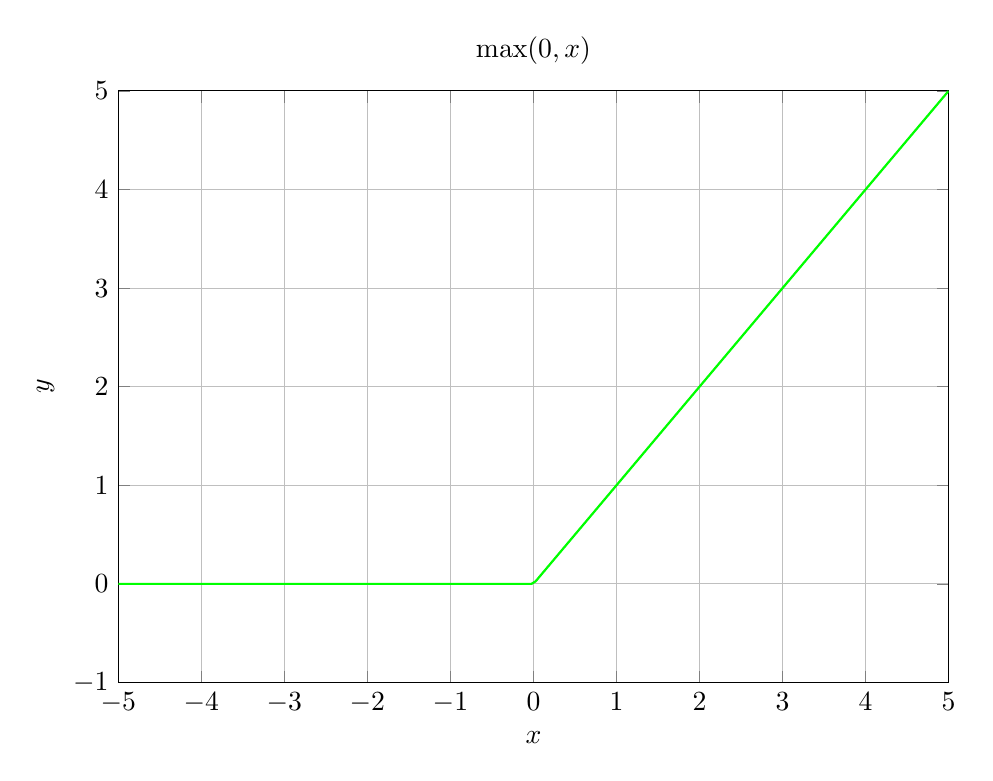
\begin{tikzpicture}
            \begin{axis}[
                title={$\max(0,x)$},
                xlabel={$x$},
                ylabel={$y$},
                grid=major,
                width=\textwidth,
                height=0.75\textwidth,
                xmin=-5, xmax=5,
                ymin=-1, ymax=5,
            ]
                \addplot[green, thick, samples=200, domain=-5:5] {max(0,x)};
            \end{axis}
        \end{tikzpicture}
    \end{minipage}
    \centering
    \caption{Three activation functions.}
\end{figure}

\subsubsection{Types}

\textit{Feedforward neural networks} (FNN) and \textit{recurrent neural networks} (RNN) are two main categories of neural networks. So far, we have been discussing FNN only, whose flow of information is uni-directional, from the input layer to the output layer, without any cycles or loops. FNN is sufficient for ordinary tasks such as regression and classification. However, for more complicated problems, RNN plays an important role. In RNN, outputs from previous steps can be fed as input to the current step, allowing it to maintain a form of ‘memory’. This makes RNN particularly effective for tasks such as time series prediction, natural language processing, and speech recognition. We will delve into RNN more deeply later.

\subsubsection{Gradient Descent}

\textit{Gradient descent} is an algorithm that helps to find the local minima of a function. Intuitively speaking, it starts at a given point and proceeds to the opposite direction of the gradient, where the function descends the most, then continues until the gradient vanishes, which is the local minimum. In the context of neural network, it is used to minimise the loss function. To solve the optimisation problem, several algorithms will be used. We will discuss this in more detail later.

\subsection{Example: Regression}

\textit{Regression} is a technique that approximates data and estimates the relationship between variables. In the context of machine learning, the dependent variable is usually called a \textit{label}. In the second year, we learnt some basics of regression: linear regression in the statistical modelling course and polynomial regression in the numerical analysis course. With the help of neural networks, we might take the idea further and explore non-linear regression.

Consider a simple example of a neural network that performs regression based on $y = \sin x$. Assume that we are given $n$ data points between $[-\pi, \pi]$, denoted by $\mathbf{x}$. We try to minimise the difference between the predicted output $f(\mathbf{x})$ and the target output $\sin (\mathbf{x})$, where $f$ is the neural network being considered.

We are now going to present an implementation of this neural network in Julia. We first need to import some packages for later use. 

\begin{verbatim}
using Lux, Random, Optimization, OptimizationOptimisers,
      ComponentArrays, Zygote, Plots, LinearAlgebra
\end{verbatim}

Then we define the data. Let us select 100 evenly spaced points from $[-\pi, \pi]$ and store them in \verb|x|. We will also define the target output in \verb|y|.

\begin{verbatim}
x = range(-pi, pi; length = 100)
y = sin.(x)
\end{verbatim}

To create the neural network model, a Julia package \verb|Lux| is usually used. For the purpose of this example, we could use three layers, all of which are \verb|Dense|, i.e., every neuron in one layer is connected to every other neuron in the next layer. For 100 data points, 10 neurons in the hidden layer would be enough. We can create the composition of such layers using the \verb|Chain| command. The input and hidden layers will have ReLU as the activation function.

\begin{verbatim}
model = Chain(
    Dense(1 => 10, relu),
    Dense(10 => 10, relu),
    Dense(10 => 1)
)
\end{verbatim}

After that, we will implement the loss function based on \verb|norm| from the \verb|LinearAlgebra| package. We might consider our loss function to be the $L^2$-norm of $f(\mathbf{x}) - \sin (\mathbf{x})$.

\begin{verbatim}
function regression_loss(ps, (model, st, (x, y)))
    return norm(vec(model(x', ps, st)[1]) - y)
end
\end{verbatim}

We now turn our attention to the optimisation problem. We can use \verb|setup| from the package \verb|Lux| to create an initial guess of the parameters and \verb|MersenneTwister| from the package \verb|Random| to make it random.

\begin{verbatim}
ps, st = Lux.setup(MersenneTwister(), model)
\end{verbatim}

To define and solve the optimisation problem, we use the aforementioned gradient descent method supplied by \verb|Adam| in \verb|OptimizationOptimisers|. To calculate the gradients needed, \verb|AutoZygote| from the \verb|Zygote| package is used. Details of these will be explored later. We also need to wrap \verb|ps| in an array type supplied in the \verb|ComponentArrays| package, as the \verb|Optimization| package requires the optimisation to be over an array type.

\begin{verbatim}
prob = OptimizationProblem(OptimizationFunction(regression_loss,
       Optimization.AutoZygote()), ComponentArray(ps), (model, st, (x, y)))
ret = solve(prob, Adam(0.03), maxiters = 250)
\end{verbatim}

Lastly, we can visualise our results by plotting supplied in the \verb|Plots| package:

\begin{verbatim}
plot(x, y, label = "True")
plot!(x, vec(model(x', ret.u, st)[1]), label = "Predicted")
\end{verbatim}

\begin{figure}[htbp]
    \centering
    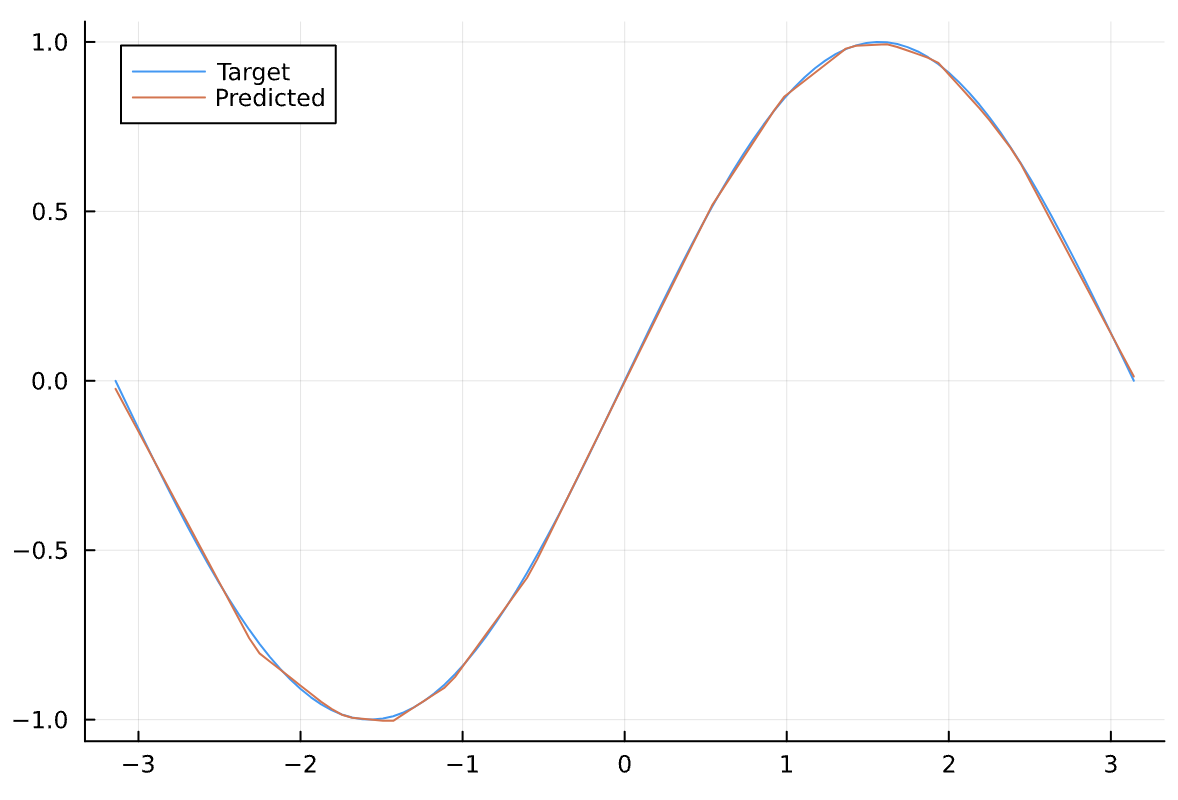
\includegraphics[width=0.8\textwidth]{figures/Regression.png}
    \caption{Regression of $y = \sin x$.}
\end{figure}

This is a pretty impressive result!

\subsection{Example: Classification}

Classification is another powerful application of neural networks. It involves using a neural network to assign labels to input data based on some patterns learnt during the training process. A classic example is digit recognition based on the \textit{MNIST database} (Modified National Institute of Standards and Technology database). This database presents a large collection of handwritten digits given in pixels. The task is to learn from the database and classify the digits.

We are now going to present an implementation of this neural network in Julia. The idea is taken from \href{https://github.com/piotrek124-1/Simple_MNIST_Julia/tree/main}{here}.

We first need to import some packages for later use. For this task, we introduce another package \verb|Flux|, which is similar to \verb|Lux| but even more powerful. 

\begin{verbatim}
using Flux, MLDatasets
\end{verbatim}

First, we import the MNIST database from the \verb|MLDatasets| package.

\begin{verbatim}
x_train, y_train = MLDatasets.MNIST.traindata(Float32)
x_test, y_test = MLDatasets.MNIST.testdata(Float32)
\end{verbatim}

We then need to ‘flatten’ the images so that they become vectors and would be easier to process. For labels, we need to use a technique called \textit{one-hot encoding} to transform categorical variables into \textit{one-hot} form, i.e., a group of bits with one and only one \verb|1| and all other bits \verb|0|.

\begin{verbatim}
x_train_flat = Flux.flatten(x_train)
x_test_flat = Flux.flatten(x_test)
dataset = [(x_train_flat, Flux.onehotbatch(y_train, 0:9))]
\end{verbatim}

After that, we define the neural network for our use. The input layer consists of $28\times 28 = 784$ neurons. We employ two hidden layers, each of which has $1/4$ the number of neurons compared to the previous layer. Finally, the output layer consists of 10 neurons corresponding to the digits 0 to 9. As usual, the ReLU activation function is used.

\begin{verbatim}
model = Chain(
    Dense(784, 196, relu),
    Dense(196, 49, relu),
    Dense(49, 10)
)
\end{verbatim}

The loss function we are using is a modified form of the \textit{cross-entropy}. It measures the performance of a classification model whose output is a probability value between $0$ and $1$. Cross-entropy loss increases as the predicted probability diverges from the actual label.

\begin{verbatim}
loss(x, y) = Flux.Losses.logitcrossentropy(model(x), y)
\end{verbatim}

We are now ready to train our neural network. For this task, it is better to train the neural network several times, or \textit{epochs}. To optimise the performance, we shall use 25 epochs.

\begin{verbatim}
for epoch in 1:25
    Flux.train!(loss, Flux.params(model), dataset, Adam(0.003))
end
\end{verbatim}

We might see the test accuracy given as

\begin{verbatim}
sum(Flux.onecold(model(x_test_flat)) .== (y_test .+ 1)) / length(y_test)
\end{verbatim}

which is normally around $80\%$. That is great but not extremely satisfying. This inspires us to consider a better model, as detailed below. 

\section{Introduction to Neural ODEs}

\subsection{Motivation}

The method of \textit{neural ODEs} (neural ordinary differential equations) was first proposed in a 2018 paper titled "Neural Ordinary Differential Equations". This paper won the Best Paper Award at NeurIPS in the same year. The inspiration for neural ODEs came from the observation of a specific neural network model called the \textit{residual neural network} (ResNet). This model was introduced by a research team at Microsoft in 2015. Unlike traditional neural networks, ResNet incorporates residual connections by adding a residual term to the output of each layer, as shown in the equations below.
\begin{equation}\label{eq1}
    h_{t+1} = h_t + \mathrm{ReLU}\left(W_t h_t + b_t\right),\tag{1}
\end{equation}
\begin{equation}\label{eq2}
    h_{t+1} = h_t + f\left(h_t, \theta_t\right).\tag{2}
\end{equation}
Here, the second term in equation \ref{eq1} is in the form of a typical neural network. To get the state at layer $t+1$, we perform calculation using the current state $h_t$, the weight matrix $\textbf{W}_t$ and bias vector $\textbf{b}_t$  at layer $t$, and a non-linear activation function ReLU. The first term of $(1)$, $h_t$ is the residual term, representing the identity of the hidden state at layer $t$.
We can write equation \ref{eq1} in the form of equation \ref{eq2}, where $f$ is a function that depends on the state at layer $t$ and some parameters related to this layer. Then, by transforming equation \ref{eq2}, we get
$$\frac{h_{t+1} - h_t }{1}= f(h_t, \theta_t),$$
which gives
$$\frac{h_{t+\Delta t} - h_t }{\Delta t}\Bigg|_{\Delta t=1}= f(h_t, \theta_t).$$
Such a form inspires us to make $\Delta t$ infinitesimally small, allowing us to transform this discrete form into a continuous one:
$$\lim_{\Delta t\to 0}\frac{h_{t+\Delta t} - h_t }{\Delta t}= f(h_t, \theta_t,t)$$
This motivates us to consider ordinary differential equations, which can be written as
\begin{equation}\label{eq3}
    \dot{h}(t)= f(h(t), \theta,t).\tag{*}
\end{equation}
This is the most important equation in neural ODE. The function $f$ on the right is a function derived from a neural network, with $\theta$ representing the parameters of that network. By convention, since there is no concept of hidden layers in neural ODE, we usually write the function \ref{eq3} as
$$\frac{\mathrm{d}z}{\mathrm{d}t}= f(z(t), \theta,t).$$

\section{Solving Neural ODEs}

\subsection{Solving Steps}

Solving differential equations is a difficult process, requiring much effort in existence theorems and techniques. Solving neural ODEs and CDEs therefore poses a significant challenge in and of itself. Having defined basic neural network and neural ODEs/CDEs theory, we now turn our attention to the steps required to solve such problems numerically.

Consider a neural ODE defined by neural networks $f$ and $g$, such that $f_\theta$, when provided with parameters $\theta$, defines the differential equation of the system $\dot{x} = f_\theta\left(t, x\right)$, and $g_\phi$, when provided with parameters $\phi$, defines the initial value of the system $x\left(t_0\right) = g_\phi(t_0)$. In order to solve the neural ODE/CDE numerically, we are required to:

\begin{enumerate}
    \item \textit{Train $g_\phi$ to predict the initial value of the system.} This requires the use of a loss function to train the neural network $g_\phi$, providing the parameters required to accurately predict the initial value of the system. 
    \item \textit{Train $f_\theta$ to provide the parameters of the neural ODE/CDE.} Similar to the prior step, this requires a loss function to train the neural network $f_\theta$, providing the parameters required to accurately state the specific ODE in question. Once the parameters have been approximated, we are left with a standard ODE problem.
    \item \textit{Solve the ODE Problem.} As most ODEs do not have analytical solutions, we make use of numerical ODE solvers to approximate the solution of the system.
\end{enumerate}

This section aims to define and discuss the methods and techniques required to perform such numerical analysis on neural ODEs/CDEs. In particular, the basic ideas of loss functions, gradient descent, and automatic differentiation are introduced here in Section 4.1. Sections 4.2 and 4.3 cover the methods used to train the relevant neural networks, and finally Section 4.4 discusses several numerical methods to solve the eventual ODEs after training.

\subsubsection{Loss Functions}
points to cover:
\begin{itemize}
    \item why we need loss functions
    \item definition of loss function
    \item how to choose loss functions
    \item basic examples
    \item what to do with loss functions?
\end{itemize}

\subsubsection{Gradient Descent and Applications}
points to cover:
\begin{itemize}
    \item motivation for gradient descent
    \item basic gradient descent and possible issues
    \item stochastic gradient descent - costly calculations
    \item adaptive gradient techniques - RMSProp, ADAM
    \item when to use what method for training
\end{itemize}

\subsubsection{Automatic Differentiation}
points to cover:
\begin{itemize}
    \item motivation behind AD
    \item starting with dual numbers
    \item extending dual numbers to higher dimensions
    \item extending dual numbers to multivariable contexts (taylor series)
    \item AD in general scenarios: chain rule
    \item julia packages implementing AD
\end{itemize}

\subsection{Backpropagation}

\subsection{log ODE Method}

\subsection{Numerical ODE Solvers}
Upon completion of training of the neural networks (where we have derived the learnt parameters $\theta$, $\phi$), all that remains is to solve the subsequent ODE numerically. This can be done in a number of methods, which are generally known as the \textit{Runge-Kutta} methods.

\subsubsection{Euler's Method}
points to cover:
\begin{itemize}
    \item motivation for euler's method
    \item definition of euler's method
    \item proof of euler's method
    \item limitations of euler's method
\end{itemize}

\subsubsection{Runge-Kutta Methods}
points to cover:
\begin{itemize}
    \item general runge-kutta methods definition (including matrix representation)
    \item euler's method is a runge-kutta method (1st order)
    \item an example: RK4 (basic? proof and full extension of definition)
    \item actual runge-kutta methods used in julia packages - 5th orders and above  
    \item a short comment on what makes a good method for solving ODEs
\end{itemize}

\section{Application (Jiankuan Liu's Part)}

\section{Extension: Neural CDEs}

\subsection{Motivation}
As we have seen before, neural networks and differential equations seem to be irrelevant but, in fact, they have been proven to be two sides of the same coin. In particular, neural ODEs can be seen as a continuous-time analogue to the ResNet. However, there exist certain real-life applications such as time series forecasting where neural ODEs are no longer effective in solving the problem. Fortunately, a famous British mathematician Terry Lyons developed a novel and exciting field of mathematics called rough path in the 1990s, and we can use some mathematical insights from this theory to develop a new concept called \textit{neural CDEs} (neural controlled differential equations).

\subsubsection{Definition}
Before defining neural CDEs, it is essential that we understand the definition of CDEs. To formally introduce it, we need to introduce a new notion of integration, the Riemann–Stieltjes integral.

\definition{(Riemann–Stieltjes integral)}
For a function $f$

\section{Conclusion}

\section*{Acknowledgments}
\addcontentsline{toc}{section}{Acknowledgement}

\appendix

\section{First appendix}

\section{Second appendix}

\bibliography{bibliography.bib}
\end{document}